\section{Metodologia testowania}
\subsection{Warunki testowe i środki zachowania bezpieczeństwa}
Ze względu na mój relatywny brak doświadczenia w sferze cyberbezpieczeństwa postanowiłem 
zachować możliwie najwyższe środki ostrożności podczas testowania scenariuszy ataku. W szczególności tyczy się to infekcji prawdziwym wirusem ransomware.\newline
Moim stanowiskiem pracy był laptop Asus TUF Gaming FX505D z 8 GB ramu i 512 GB pamięci nvme z zainstalowanym linuksem Proxmox VE 8.1\footnote{Obraz systemu został pobrany ze strony \url{https://www.proxmox.com/en/downloads}. SHA256 obrazu wynosiło 9018a17307ad50eb9bf32a805d0917d621499363ef87b0b477332ed9f9d7dcc1.}. Proxmox jest dystrybucją specjalizującą się wirtualną infrastrukturą (na rodzaj VmWare). Posiada ona wygodny interfejs graficzny dostępny przez sieć oraz dużo udogodnień w dziedzinie wirtualizacji.
\newline
Wszystkie testowane maszyny wirtualne mają zainstalowane na sobie Ubuntu Server 22.04 LTS\footnote{\url{https://ubuntu.com/download/server}}. Każda wirtualna maszyna ma przydzielone 32 GB pamięci twardej, 8GB pamięci ram oraz 8 procesorów. Jako hypervisor korzystałem z QEMU\footnote{\url{https://www.qemu.org/}} bez KVM\footnote{\url{https://linux-kvm.org/page/Main_Page}} o czym opowiem krótko za chwilę.
\begin{figure}[H]
    \centering
    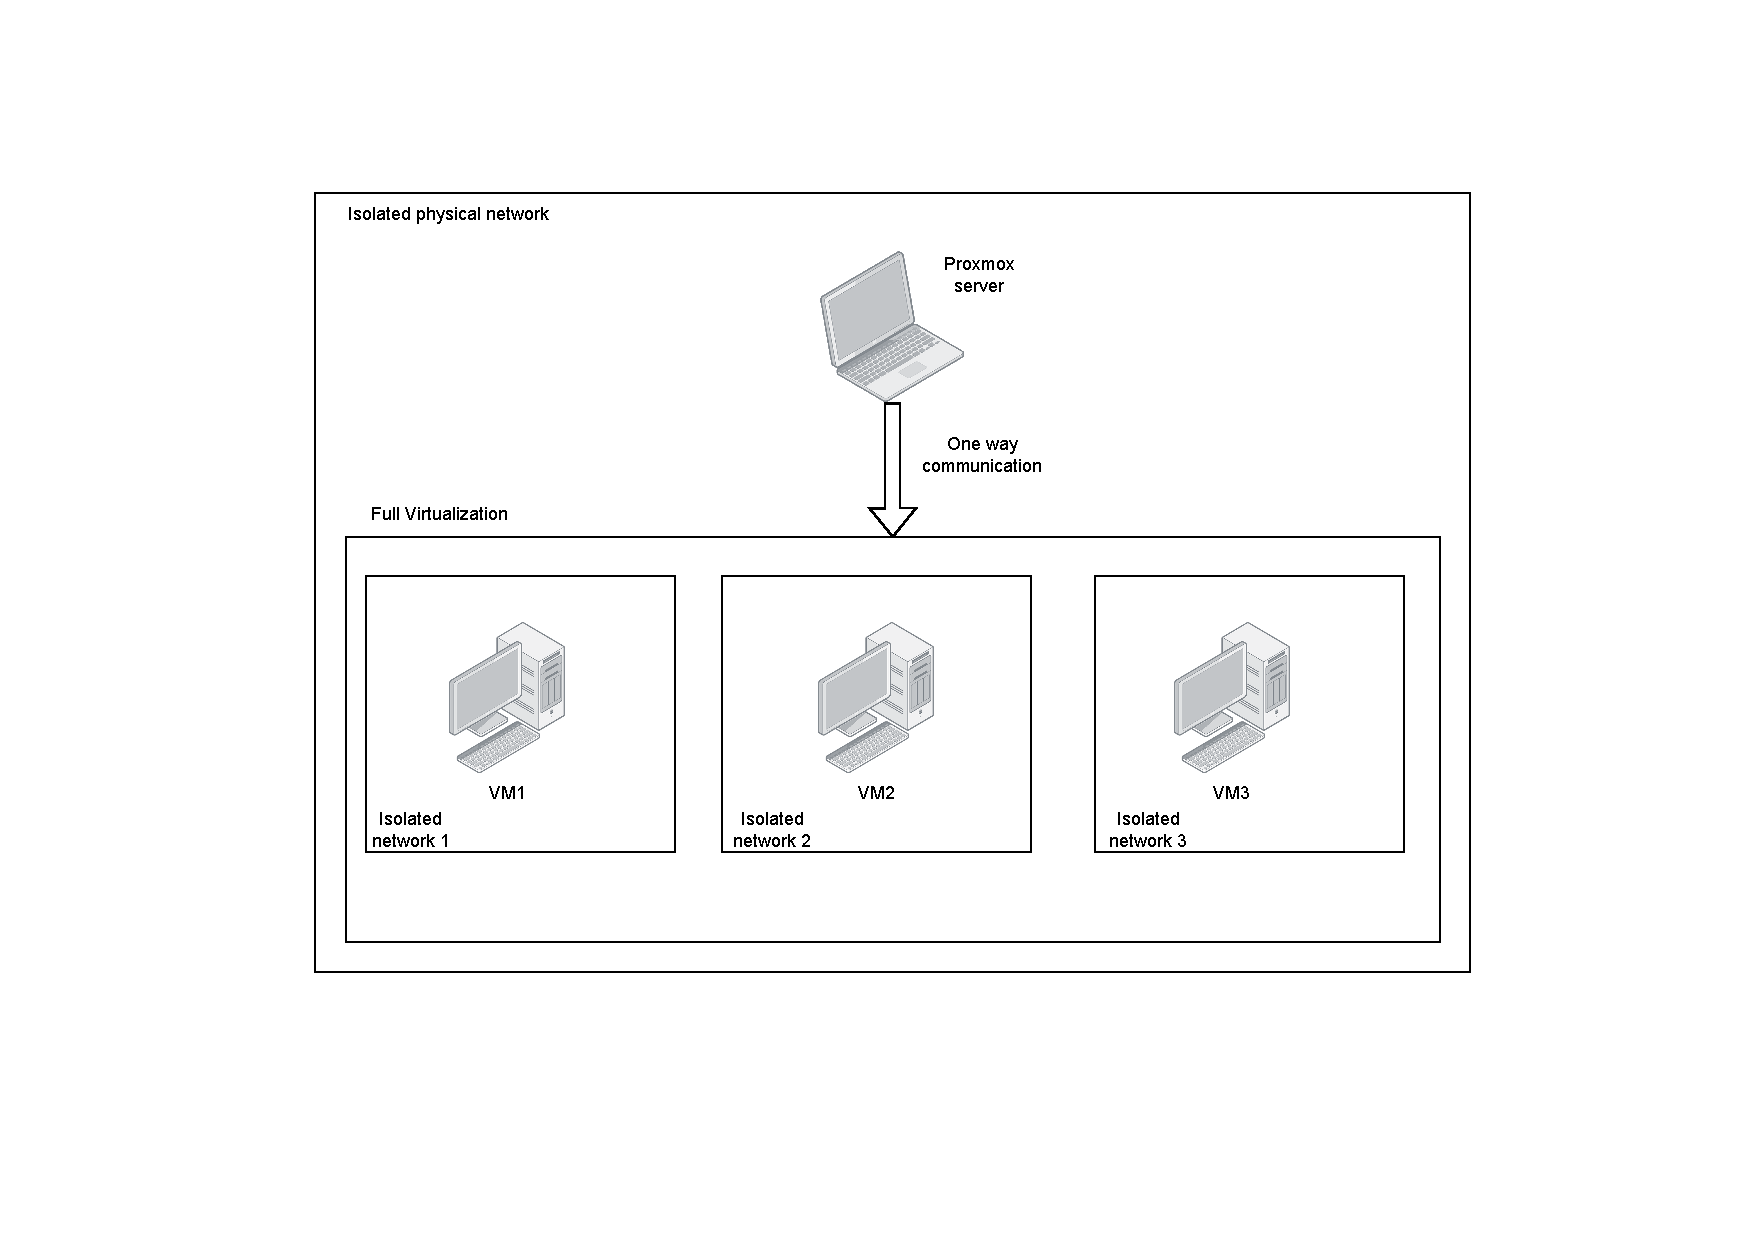
\includegraphics[width=0.45\linewidth]{rysunki/test.drawio.pdf}
    \caption{Architektura infrastruktury testowej.}
    \label{fig:enter-label}
\end{figure}
Mimo iż użycie KVM sprawiłoby, że maszyny wirtualne działałyby znacznie szybciej niż w wypadku pełnej wirtualizacji, to nie użyłem tego rozwiązania z powodu braku konkretnych dowodów na absolutne bezpieczeństwo KVM switcha na oprogramowanie złośliwe. Dodatkowymi środkami bezpieczeństwa było zupełne wyizolowanie wirtualnych maszyn we własnych sieciach na maszynie, która z kolei była kompletnie fizycznie wyizolowana od sieci zewnętrznych.

\subsection{Ustalenie metryki skuteczności rozwiązania}
Podstawowym założeniem testowania skuteczności rozwiązania, było to, że testy muszą mieć w sobie elementy ataku. W tym wypadku nie ma sensu testowanie skuteczności jako dokładności wykrywania obecności ataku, gdyż jest on elementem stałym wszystkich scenariuszy. Zamiast tego postanowiłem, że skuteczność rozwiązania będzie mierzona na podstawie \emph{czasu wykrycia} od momentu rozpoczęcia ataku. Wydaje mi się to miarodajnym rozwiązaniem, naturalnie powiązanym z potencjalnymi stratami w organizacji.
\newline
Niestety średni czas wykrycia ataku według raportu IBMu w 2018 roku wyniósł 197 dni, a w 2019 - 207 dni. Aby test był wykonywalny w sensownym czasie nie mogłem sobie pozwolić na aż tak długi okres próbny. Z powodu zaistniałej sytuacji postanowiłem zaproponować subiektywnie wybraną miarę, której wielkość motywowałem niewielkim rozmiarem systemów użytych w testach. Mianowicie - \textbf{jeśli na 10 godzin od rozpoczęcia ataku zostanie wykryte potencjalne zagrożenie, to test został zakończony sukcesem}. W przeciwnym wypadku doszło do porażki. 
%%%%%%%%%%%%%%%%%%%%%%%%%%%%%%%%%%%%%%%%%%%%%%%%%%%%%%%%%%%%%%%%%%%%%%%%%%%%%%%%%%%%
\section{Scenariusze testowe symulujące ataki ransomware}
\subsection{Improwizowany atak z kompresowaniem}
Jako podstawowy scenariusz ataku postanowiłem dokonać archiwizacji z szyfrowaniem na ścieżce z milionem plików. Atak miał na celu zaszyfrowanie wyłącznie plików z rozszerzeniem, \texttt{.txt}. W tym samym miejscu obecne były również pliki o innych rozszerzeniach.
\begin{lstlisting}[language=bash,
    backgroundcolor=\color{EEGold!5!white},
    caption={Komenda użyta do wykonania "ataku".},
    label={lst:commau}]
    $ zip --encrypt files.zip *.txt
    $ rm -f *.txt
\end{lstlisting}
Warto dodać, że komenda nie wymagała przywilejów super usera. Istnieje więc możliwość wystąpienia ataku w organizacji w której doszło do wycieku danych kont pracowników bez przywilejów sudo.
\begin{lstlisting}[language=bash,
    backgroundcolor=\color{EEGold!5!white},
    caption={Fragment logów z części audytowej. Będzie to jedyny tak długi fragment, który
    chciałem pokazać w celach informacyjnych.},
    label={lst:logau}]
    2023-12-17T22:33:07.316Z INFO  [linux_fs_audit] Inserting {"user":"maciek","group":"maciek","executable":"/usr/bin/rm","syscall":"unlinkat","timestamp":"1702852387","key":"WRITE"}
    2023-12-17T22:33:07.351Z INFO  [linux_fs_audit] Unix stream is readable.
    2023-12-17T22:33:07.351Z INFO  [linux_fs_audit] Unix stream is readable.
    2023-12-17T22:33:07.351Z WARN  [linux_fs_audit] Blocking error while reading from socket
    2023-12-17T22:33:09.762Z INFO  [linux_fs_audit] Unix stream is readable.
    2023-12-17T22:33:09.762Z INFO  [linux_fs_audit] Opening an Sqlite connection
    2023-12-17T22:33:09.763Z INFO  [linux_fs_audit] Inserting {"user":"maciek","group":"maciek","executable":"/usr/bin/bash","syscall":"openat","timestamp":"1702852389","key":"READ"}
    2023-12-17T22:33:09.781Z INFO  [linux_fs_audit] Opening an Sqlite connection
    2023-12-17T22:33:09.792Z INFO  [linux_fs_audit] Unix stream is readable.
    2023-12-17T22:33:09.792Z WARN  [linux_fs_audit] Blocking error while reading from socket
    2023-12-17T22:33:12.999Z INFO  [linux_fs_audit] Unix stream is readable
    2023-12-17T22:33:12.999Z INFO  [linux_fs_audit] Opening an Sqlite connection
    2023-12-17T22:33:12.999Z INFO  [linux_fs_audit] Inserting {"user":"maciek","group":"maciek","executable":"/usr/bin/zip","syscall":"openat","timestamp":"1702852392","key":"WRITE"}
    2023-12-17T22:33:13.028Z INFO  [linux_fs_audit] Opening an Sqlite connection
    2023-12-17T22:33:13.053Z INFO  [linux_fs_audit] Unix stream is readable.
    2023-12-17T22:33:13.053Z INFO  [linux_fs_audit] Opening an Sqlite connection
    2023-12-17T22:33:13.053Z INFO  [linux_fs_audit] Inserting {"user":"maciek","group":"maciek","executable":"/usr/bin/zip","syscall":"unlink","timestamp":"1702852393","key":"WRITE"}
    2023-12-17T22:33:13.100Z INFO  [linux_fs_audit] Opening an Sqlite connection
\end{lstlisting}
Logi z części audytowej dobrze ukazują zakres działania tego komponentu aplikacji. W trybie informacyjnym można zauważyć przewijanie linijek z informacjami o odczytanych operacjach. Dodatkowo można zauważyć status odczytu z gniazda \texttt{auditd} oraz informacje o zapisie danych o operacji do bazy Sqlite w tym operacje w notacji JSON.

\begin{lstlisting}[language=bash,
    backgroundcolor=\color{EEGold!5!white},
    caption={Raport wygenerowany ze skanera, który pozwoliłem sobie delikatnie sformatować aby widać było lepiej jego treść.},
    label={lst:raportau}]
    <9>1 2023-12-18T18:11:20.485Z
    test-hostname 
    ransomware-scanner 
    - - -  
    Strategy evaluations: {
    "Executable":"Low",
    "Threshold":"High",
    "Rename":"Low",
    "RansomNote":"Low"
}
File risk evaluation {
    "/home/maciek/box/testfile.png":"High",
    "/home/maciek/box/h1.csv":"Medium",
    "/home/maciek/box/files.zip":"High",
    "/home/maciek/box/h2.csv":"Medium"
}
\end{lstlisting}
W raporcie można zobaczyć, że jedyną metodą, która wykryła podejrzany ruch na maszynie była strategia z przekroczeniem ustalonej ilości operacji na jednostkę czasu. W wypadku tej maszyny było to 300 operacji na 100 ms. Czas wykrycia pokrył się z interwałem inicjalizacji analizy i wyniósł ok \textbf{167 ms}.
\subsection{Atak Ransom EXX}
\subsection{Atak Erebus}
\section{Analiza działań systemu i statystyk generowanych podczas symulowanego ataku}
\section{Ewaluacja skuteczności wykrywania}
